% generated by Docutils <http://docutils.sourceforge.net/>
\documentclass[t,english]{beamer}
\usepackage{hyperref}

\definecolor{rrblitbackground}{rgb}{0.55, 0.3, 0.1}

\newenvironment{rtbliteral}{

\begin{ttfamily}

\color{rrblitbackground}

}{

\end{ttfamily}

}

\usetheme{Warsaw}

\setbeameroption{hide notes}

\usepackage{fixltx2e} % LaTeX patches, \textsubscript
\usepackage{cmap} % fix search and cut-and-paste in PDF
\usepackage[T1]{fontenc}
\usepackage[latin1]{inputenc}
\usepackage{ifthen}
\usepackage{babel}
\usepackage{graphicx}

%%% Custom LaTeX preamble
% PDF Standard Fonts
\usepackage{mathptmx} % Times
\usepackage[scaled=.90]{helvet}
\usepackage{courier}

%%% User specified packages and stylesheets

%%% Fallback definitions for Docutils-specific commands

% hyperlinks:
\ifthenelse{\isundefined{\hypersetup}}{
  \usepackage[unicode,colorlinks=true,linkcolor=blue,urlcolor=blue]{hyperref}
  \urlstyle{same} % normal text font (alternatives: tt, rm, sf)
}{}

%%% Body
\begin{document}

\begin{frame}[fragile]
\frametitle{Simple columns}

\begin{columns}[T]
\column{0.47\textwidth}

\noindent\makebox[\textwidth][c]{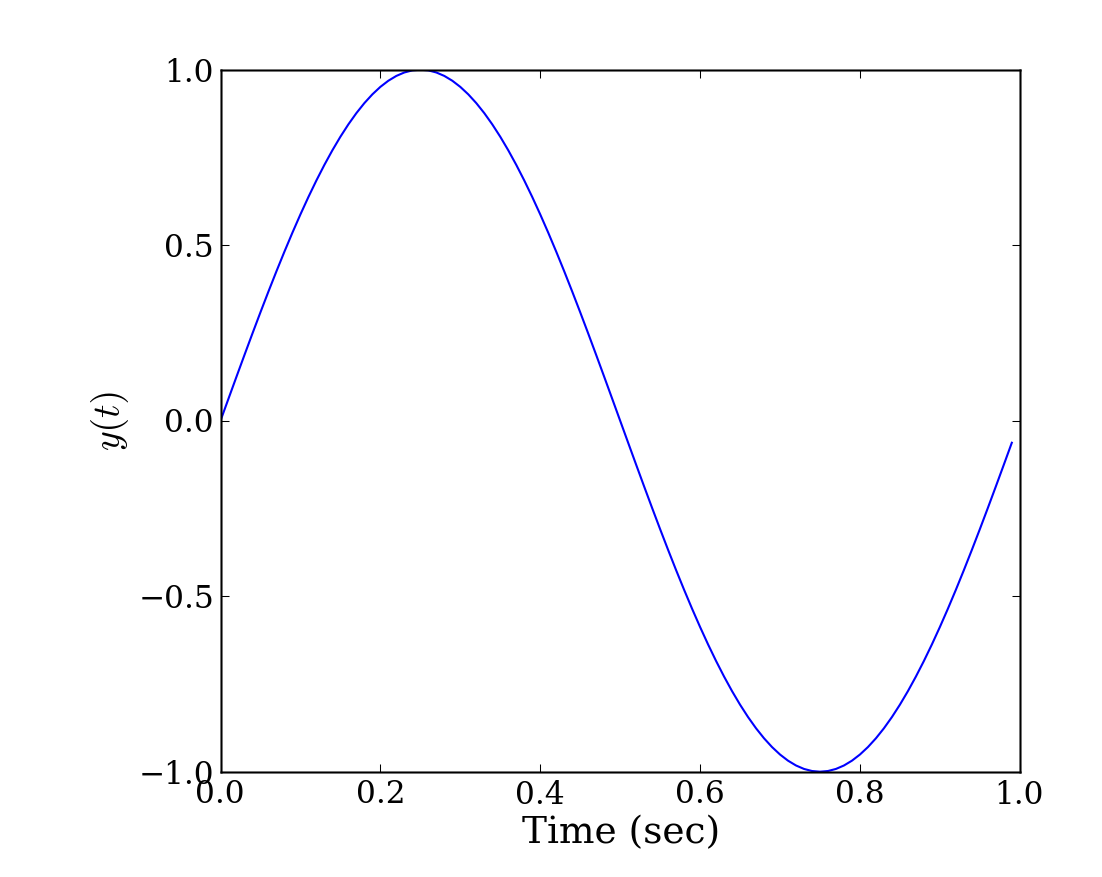
\includegraphics[width=1.300\linewidth]{plot.png}}

\column{0.47\textwidth}
\begin{itemize}[<+-| alert@+>]

\item bullet 1

\item bullet 2

\item bullet 3
\end{itemize}

\end{columns}
\end{frame}

\begin{frame}[fragile]
\frametitle{Explicit columns}

\begin{columns}[T]
\column{0.75\textwidth}

\noindent\makebox[\textwidth][c]{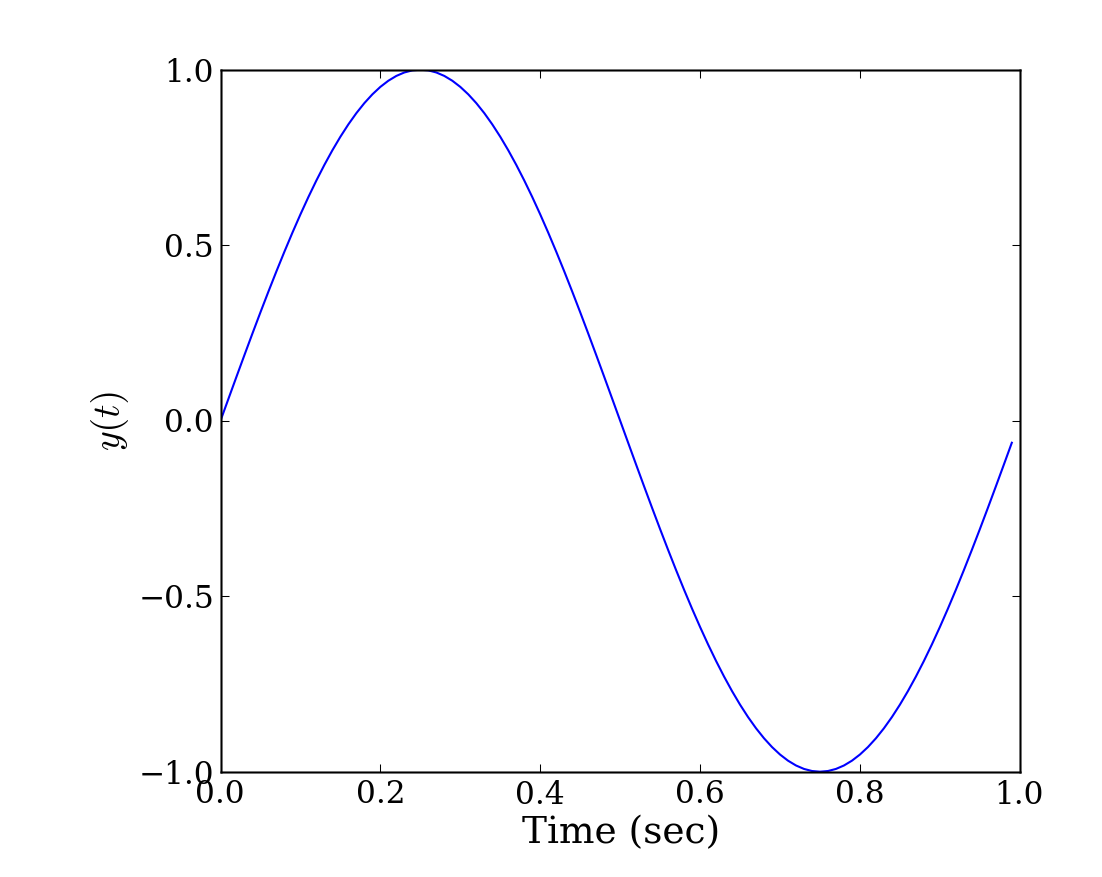
\includegraphics[height=0.75\textheight]{plot.png}}

\column{0.20\textwidth}
\begin{itemize}[<+-| alert@+>]

\item bullet 1

\item bullet 2

\item bullet 3
\end{itemize}

\end{columns}
\end{frame}

\begin{frame}[fragile]
\frametitle{A slide without columns}


Just to make sure our ``columnization'' isn't persistent, this should show up
up as a plain normal slide.
\end{frame}

\end{document}
